% =============================================================================
% Chuong 6: Platform demo (chuan lop article cho Internship2_HK262)
% Nguon noi dung: docs/drafts/ch6-demo-platform.md, outline-bao-cao-gd2.md (Ch6),
%   eval/results/{pipeline_val_v2,pipeline_test_v2,pipeline_sens_test_v1}/runtime.json,
%   eval/results/m10_demo_cases_v1/demo_cases.json, docs/milestones/M11-danh-gia-nguoi.md
% Nhan dung tu chuong khac: ch:de-xuat, ch:thuc-nghiem, ch:thao-luan,
%   sec:ch4-c1, sec:ch4-policy, sec:ch4-rca, sec:ch4-grouping, sec:ch4-propagation,
%   sec:ch4-report, sec:ch4-impl, sec:ch2-cong-nghe, sec:ch5-rca-results,
%   sec:ch5-finding11, tab:ch5-findings, tab:ch5-verdict-summary
% =============================================================================

\section{Platform demo}
\label{ch:platform}

Chương này trả lời câu hỏi liệu toàn bộ chuỗi xử lý ở Chương~\ref{ch:de-xuat}, từ bộ phát hiện bất thường qua \CTAV{} tới tác tử \term{RCA}{RCA}, có vận hành được thành một hệ thống điều hành trực quan mà kỹ sư trực ca và hội đồng thẩm định dùng được hay không. Chương không đưa ra kết quả thực nghiệm mới; mọi con số đều đọc lại từ các lượt chạy đã đóng băng ở Chương~\ref{ch:thuc-nghiem}. Mục~\ref{sec:ch6-vai-tro} xác định vai trò, phạm vi và cơ chế tách lớp hiển thị của platform. Mục~\ref{sec:ch6-luong} mô tả luồng dữ liệu đầu--cuối, tám endpoint chỉ đọc và kiến trúc triển khai bằng Docker Compose. Mục~\ref{sec:ch6-dashboard} đi qua năm màn hình theo trình tự thao tác thực tế, Mục~\ref{sec:ch6-kich-ban} trình bày kịch bản demo năm phút, và Mục~\ref{sec:ch6-kiem-thu} báo cáo kết quả kiểm thử ngoại tuyến cùng phương án dự phòng không phụ thuộc Docker.

% -----------------------------------------------------------------------------
\subsection{Vai trò của platform}
\label{sec:ch6-vai-tro}

Mục này làm rõ platform được xây để chứng minh điều gì và chủ đích giới hạn ở đâu. Platform là hiện thực chạy được của \CTAV{} và tác tử \term{RCA}{RCA}: cùng một pipeline vừa xuất các tệp kiểm định \hyp{H0}--\hyp{H5}, vừa nạp dữ liệu cho giao diện điều hành. Nhờ vậy, bất kỳ cảnh báo, sự cố hay nút đồ thị nào hiển thị trên màn hình cũng đối ứng một--một với bản ghi trong kho kết quả của Chương~\ref{ch:thuc-nghiem}, không tồn tại dữ liệu mô phỏng riêng cho trình diễn. Giao diện tách bạch hai chế độ quan sát qua công tắc trên thanh công cụ: chế độ vận hành (\emph{Ops View}) ẩn hoàn toàn nhãn lỗi chuẩn để phản ánh đúng thông tin mà người trực ca nhìn thấy, trong khi lớp phủ đánh giá (\emph{Eval Overlay}) bật đường lỗi chuẩn Nezha và huy hiệu đối chiếu đúng/sai phục vụ hội đồng kiểm chứng. Vì mục tiêu ưu tiên tính tái lập khoa học thay vì vận hành thương mại, hệ thống không cài đặt xác thực người dùng, không phân quyền đa thuê bao, không bắn thông báo ra ngoài và không tự động thực thi kịch bản khắc phục.

Ràng buộc thiết kế thứ hai là toàn bộ buổi trình diễn phải vận hành độc lập khi ngắt hoàn toàn Internet. Mọi phán quyết của judge \code{gemini-2.5-flash} và mọi báo cáo chẩn đoán đều đọc lại từ bộ nhớ đệm (\code{cache}) trên đĩa theo khóa băm ở Mục~\ref{sec:ch4-judge}. Khi bật cờ \code{DEMO\_OFFLINE=1}, pipeline xóa ngay các biến khóa API khỏi tiến trình sau bước nạp cấu hình; nếu phát sinh dù chỉ một truy vấn hụt cache, tiến trình lập tức báo lỗi dừng thay vì âm thầm gọi mạng. Ứng dụng web cũng đóng gói cục bộ toàn bộ biểu tượng vector, bảng màu và mã nguồn, không tải phông chữ hay thư viện từ máy chủ bên ngoài.

% -----------------------------------------------------------------------------
\subsection{Luồng end-to-end và triển khai}
\label{sec:ch6-luong}

Mục này trình bày đường đi của dữ liệu từ tệp quan sát tới giao diện người dùng và cách bố trí các thành phần trên máy trình diễn. Luồng xử lý tuân thủ đúng thứ tự kiến trúc ở Hình~\ref{fig:ch4-arch}. Bộ phát lại đưa từng cửa sổ \code{metric} 60 giây vào bộ phát hiện \term{IF}{Isolation Forest}; các \code{candidate} vượt ngưỡng $0{,}85$ đi qua \CTAV{} gồm \comp{C1} (truy xuất lai \term{BM25}{BM25}--topology), judge \term{LLM}{LLM} đọc từ cache và chính sách quyết định có \comp{C3} (neo bằng chứng theo ngưỡng nền $p_{90}$ của \splitname{dev}). Hai thành phần \comp{C2} (ngưỡng bất đối xứng theo nguồn bằng chứng) và \comp{C4} (định tuyến hai tầng thích nghi) đã bị loại sau kiểm định trên \splitname{val}, còn \comp{C5} (\term{RescueScore}{Rescue Score}) chỉ dùng cho phân tích ablation, nên cả ba không kích hoạt trên luồng chính. Các cảnh báo giữ nhãn \code{TRUE\_ALERT} tiếp tục đi sang tác tử \term{RCA}{RCA} để gom cụm trong cửa sổ $T_{\text{group}} = 180\,\text{s}$, bỏ phiếu lan truyền ngược một bước trên đồ thị gọi và sinh báo cáo JSON có kiểm duyệt (Mục~\ref{sec:ch4-rca}).

Hình~\ref{fig:ch6-deploy} minh họa sơ đồ triển khai thực tế. Người đọc cần chú ý đường ranh giới nét đứt: bốn dịch vụ chạy thường trực trong Docker Compose, còn pipeline nạp dữ liệu chạy một lần trên máy chủ từ kho kết quả và cache đã khóa. ClickHouse lưu trữ toàn bộ \code{candidate}, phán quyết trước và sau chính sách cùng các sự kiện bằng chứng kèm điểm thành phần \term{FusionScore}{Fusion Score}; PostgreSQL lưu danh mục lượt chạy, sự cố và báo cáo chẩn đoán. Máy chủ FastAPI cung cấp tám endpoint chỉ đọc, được giao diện React/Vite truy cập qua proxy nội bộ. Các container khởi chạy theo chuỗi kiểm tra sức khỏe tuần tự: API chỉ mở cổng khi cả hai cơ sở dữ liệu đã sẵn sàng, và giao diện web chỉ nhận kết nối sau khi API phản hồi ổn định.

\begin{figure}[htbp]
  \centering
  \resizebox{\linewidth}{!}{%
  \begin{tikzpicture}[
    font=\small,
    box/.style={draw=black!75, rounded corners=2pt, align=center, text width=23mm,
                minimum height=13mm, inner sep=2pt, line width=0.6pt, fill=white},
    ctr/.style={box, draw=blue!55!black},
    flow/.style={-{Stealth[length=2mm]}, line width=0.7pt, draw=black!75},
    lab/.style={font=\scriptsize, text=black!60, align=center},
  ]
    % Phia may chu
    \node[box] (res)   at (0,1.7)  {\textbf{Kết quả đã khóa}\\[1pt]\scriptsize\texttt{eval/results/}};
    \node[box] (cache) at (0,-1.7) {\textbf{Cache LLM}\\[1pt]\scriptsize\texttt{data/llm\_cache/}\\ 0 lần gọi API};
    \node[box] (pipe)  at (3.5,0)  {\textbf{Pipeline}\\[1pt]\scriptsize nạp lại từ cache\\ \texttt{DEMO\_OFFLINE=1}};
    % Docker Compose
    \node[ctr] (ch)  at (7.1,1.7)  {\textbf{ClickHouse}\\[1pt]\scriptsize candidate, bằng chứng\\ cổng 8123};
    \node[ctr] (pg)  at (7.1,-1.7) {\textbf{PostgreSQL}\\[1pt]\scriptsize sự cố, báo cáo\\ cổng 5432};
    \node[ctr] (api) at (10.5,0)   {\textbf{API FastAPI}\\[1pt]\scriptsize 8 endpoint chỉ đọc\\ cổng 8000};
    \node[ctr] (web) at (13.9,0)   {\textbf{Dashboard}\\[1pt]\scriptsize React/Vite\\ cổng 5173};
    \node[box] (br)  at (17.3,0)   {\textbf{Trình duyệt}\\[1pt]\scriptsize người vận hành,\\ hội đồng};
    \draw[dashed, draw=blue!55!black, line width=0.7pt, rounded corners=3pt]
      (5.45,-2.75) rectangle (15.55,3.25);
    \node[font=\footnotesize\bfseries, text=blue!55!black, anchor=north west]
      at (5.55,3.2) {Docker Compose, hồ sơ \texttt{dev}};
    % Luong
    \draw[flow] (res) -- (pipe);
    \draw[flow] (cache) -- (pipe);
    \draw[flow] (pipe) -- node[lab, above, sloped]{ghi} (ch);
    \draw[flow] (pipe) -- node[lab, below, sloped]{ghi} (pg);
    \draw[flow] (ch) -- node[lab, above, sloped]{đọc} (api);
    \draw[flow] (pg) -- node[lab, below, sloped]{đọc} (api);
    \draw[flow] (api) -- node[lab, above]{\texttt{/api}} (web);
    \draw[flow] (web) -- node[lab, above]{HTTP} (br);
    \draw[flow, dashed] (res.north) -- ++(0,1.75) -| node[lab, above, pos=0.25]{bảng \hyp{H0}--\hyp{H5} tĩnh \& snapshot dự phòng, đóng gói khi dựng giao diện} (web.north);
  \end{tikzpicture}}
  \par\vspace{0.4cm}
  \caption[Sơ đồ triển khai platform bằng Docker Compose]{Sơ đồ triển khai ngoại tuyến bốn dịch vụ lưu trữ, API và giao diện từ kho kết quả đã khóa bằng Docker Compose. \emph{(Nguồn: tác giả vẽ, có hỗ trợ AI.)}}
  \label{fig:ch6-deploy}
\end{figure}

Bảng~\ref{tab:ch6-endpoints} liệt kê tám endpoint của máy chủ API cùng màn hình tiêu thụ tương ứng. Điểm thiết kế cần lưu ý là hai màn hình thuộc phân khu đánh giá (Benchmark và Methodology) không truy vấn cơ sở dữ liệu lúc chạy: bảng tổng hợp \hyp{H0}--\hyp{H5} được kết xuất tĩnh bằng script trực tiếp từ các tệp kết quả của Chương~\ref{ch:thuc-nghiem} và kiểm khớp tự động, loại bỏ hoàn toàn nguy cơ sai lệch số liệu do truy vấn giao diện. Trên lượt chạy chính thức \code{pipeline\_test\_v2}, cả tám endpoint đều phản hồi dưới một giây, bao gồm truy vấn \code{GET /alerts} trả trọn $13.699$ \code{candidate} và \code{GET /topology} tổng hợp trạng thái trên toàn bộ $56$ service cùng $68$ cạnh gọi. % src: pipeline_test_v2, tests/test_api.py

\begin{table}[H]
  \centering
  \caption[Tám endpoint của API chỉ đọc và màn hình sử dụng]{Tám endpoint của API chỉ đọc, nội dung trả về và các màn hình giao diện sử dụng.}
  \label{tab:ch6-endpoints}
  \tblfont
  \tblsetup
  \setlength{\tabcolsep}{4pt}
  \begin{tabularx}{\linewidth}{|>{\raggedright\arraybackslash}p{4.3cm}|Y|>{\raggedright\arraybackslash}p{3.5cm}|}
    \hline
    \rowcolor{gray!15}
    \textbf{Endpoint} & \textbf{Dữ liệu trả về} & \textbf{Màn hình dùng} \\
    \hline
    \code{GET /health} & Trạng thái sẵn sàng của máy chủ API & Thanh trạng thái hệ thống \& Docker healthcheck \\
    \hline
    \code{GET /runs} & Danh mục luồng cảnh báo và phiên lưu trữ sự cố kèm số lượng cửa sổ & Bộ chọn luồng dữ liệu (mọi màn hình) \\
    \hline
    \code{GET /runs/\allowbreak\{run\_id\}/metrics} & Chỉ số tổng hợp kèm CI95 của lượt chạy, khớp tệp \code{metrics.json} & Kiểm thử hợp đồng tự động, tra cứu \\
    \hline
    \code{GET /topology} & Đồ thị phụ thuộc phân tách theo phân hệ, trạng thái sức khỏe, số cảnh báo giữ lại/bị chặn và số sự cố mỗi service & Operations (\code{/overview}) \\
    \hline
    \code{GET /alerts} & Danh sách \code{candidate} theo thời gian kèm phán quyết thô, phán quyết cuối và cờ hạ bậc chính sách & Operations, Alert Stream (\code{/timeline}) \\
    \hline
    \code{GET /alerts/\allowbreak\{alert\_id\}} & Chuỗi điểm bất thường, lập luận của judge, bảng kiểm tra chính sách, vùng tìm 2-hop và điểm thành phần \term{FusionScore}{Fusion Score} & Alert Detail (\code{/alerts/\_}) \\
    \hline
    \code{GET /incidents} & Danh sách cụm sự cố đã gom nhóm trong cửa sổ $180\,\text{s}$ kèm service gốc dự đoán & Operations, Incidents (\code{/incidents}), Alert Stream \\
    \hline
    \code{GET /incidents/\allowbreak\{incident\_id\}} & Cảnh báo thành viên, đồ thị lân cận có hướng, phiếu bầu lan truyền và báo cáo chẩn đoán JSON & Incident Detail (\code{/incidents/\_}) \\
    \hline
  \end{tabularx}
\end{table}

% -----------------------------------------------------------------------------
\subsection{Dashboard điều hành và đánh giá năm màn hình}
\label{sec:ch6-dashboard}

Mục này đi qua năm màn hình của giao diện theo đúng quy trình làm việc của kỹ sư trực hệ thống và hội đồng đánh giá: quan sát toàn cảnh đồ thị phụ thuộc, theo dõi dòng cảnh báo phát lại và hàng đợi sự cố, mổ xẻ một cảnh báo đơn lẻ, điều tra một sự cố đa service, rồi đối chiếu bảng kiểm định \hyp{H0}--\hyp{H5}. Thanh điều hướng cố định bên trái chia giao diện thành hai phân khu rõ rệt là \emph{Operations} (gồm \code{Operations}, \code{Incidents}, \code{Alert Stream}) và \emph{Evaluation} (gồm \code{Benchmark}, \code{Methodology}), kèm trình khởi chạy nhanh năm kịch bản mẫu (\emph{Guided Scenarios}). Thanh lệnh phía trên giữ cố định bộ chọn luồng dữ liệu trên URL (\code{?run\_id=}), nút bật tắt lớp phủ nhãn chuẩn (\emph{Ops View} / \emph{Eval Overlay}) và nút chuyển giao diện nền giấy kem sáng hoặc nền tối vận hành. Toàn bộ nhãn trên màn hình dùng tiếng Anh để khớp chính xác với tên trường trong kho kết quả; phần phân tích dưới đây trình bày bằng tiếng Việt theo ba ý cho mỗi màn hình: ảnh chụp thực tế, câu hỏi vận hành được giải quyết và mối liên hệ với các thành phần ở Chương~\ref{ch:de-xuat}.

\subsubsection{Operations: trung tâm điều hành và đồ thị phụ thuộc toàn hệ}
\label{sec:ch6-overview}

Hình~\ref{fig:ch6-overview} là màn hình mở đầu \emph{Operations Command Center} (\code{/overview}) trên luồng kiểm thử chính thức \code{pipeline\_test\_v2} ở chế độ vận hành (\emph{Ops View}). Người đọc nên quan sát dải bốn thẻ chỉ số ở hàng trên trước, sau đó nhìn sang bản đồ phụ thuộc dịch vụ (\emph{Service Dependency Topology}) ở khung trái và danh sách sự cố ưu tiên (\emph{Priority Incident Feed}) ở khung phải.

\begin{figure}[htbp]
  \centering
  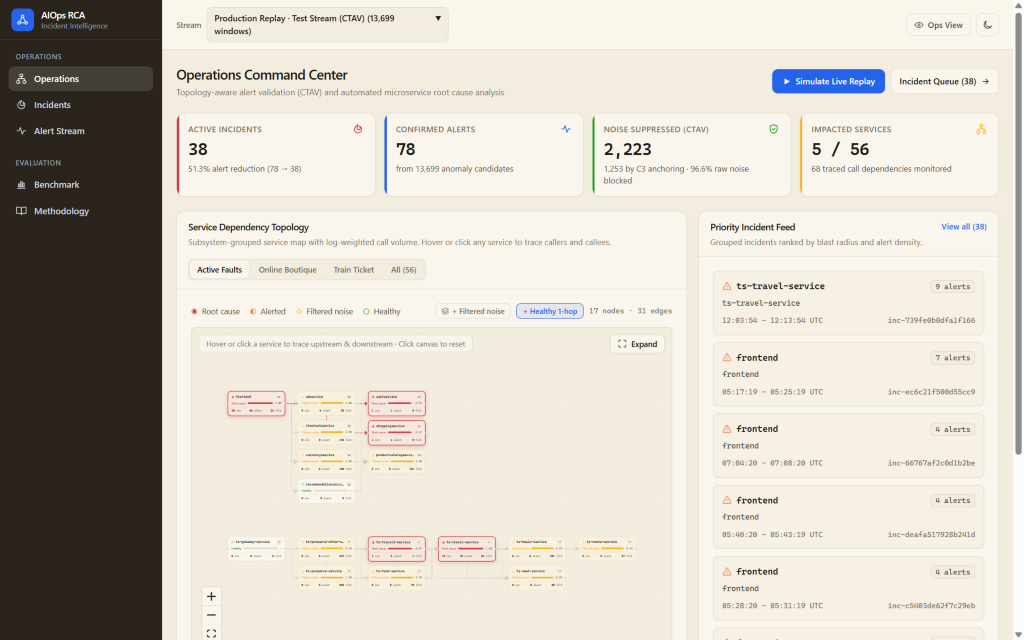
\includegraphics[width=\linewidth]{Images/C1/figures/m10-overview.png}
  \par\vspace{0.4cm}
  \caption[Màn hình Operations Command Center trên tập test]{Màn hình Operations Command Center giám sát đồ thị phụ thuộc 56 service và hàng đợi sự cố trên tập \splitname{test} (\code{pipeline\_test\_v2}).}
  \label{fig:ch6-overview}
\end{figure}

Màn hình trả lời câu hỏi định hướng đầu tiên của ca trực: \emph{trên toàn hệ thống microservice, những service nào đang phát sinh sự cố, bán kính ảnh hưởng trên đồ thị gọi rộng đến đâu và bộ thẩm định đã lọc bớt bao nhiêu nhiễu trước khi đẩy vào hàng đợi xử lý?} Trên lượt chạy \splitname{test}, bốn thẻ đầu trang cho thấy từ $13.699$ \code{candidate} bất thường, \CTAV{} chặn $2.223$ phán quyết dương tính thô ($96{,}6\%$, riêng \comp{C3} chặn $1.253$ ca), chỉ giữ lại $78$ cảnh báo xác nhận trên $5/56$ service và gom tiếp thành $38$ sự cố (mức giảm cảnh báo \term{ARR}{ARR} toàn cục đạt $51{,}3\%$). % src: pipeline_test_v2, rca_final_test_v1
Bản đồ đồ thị phân cụm tự động hai hệ OnlineBoutique và TrainTicket, quy đổi lưu lượng lời gọi theo thang logarit thành độ dày nét vẽ, đồng thời cung cấp bộ lọc nhanh theo vùng lỗi đang hoạt động (\emph{Active Faults}, rút gọn còn $17$ nút và $31$ cạnh lân cận 1-hop) cùng chế độ phóng toàn màn hình. Khi người vận hành nhấp chọn một nút bất kỳ trên đồ thị, ngăn tra cứu bên dưới lập tức liệt kê các service gọi đến (\emph{upstream callers}) và các service bị gọi (\emph{downstream callees}) để chuyển thẳng sang dòng cảnh báo đã lọc theo đúng service đó.

Về mặt phương pháp, màn hình này trực quan hóa trực tiếp đồ thị phụ thuộc \code{ServiceGraph} ($56$ nút, $68$ cạnh dựng từ trace) vốn đóng vai trò hạt nhân cho cả bước mở rộng vùng tìm 2-hop của \comp{C1} (Mục~\ref{sec:ch4-c1}) lẫn bước gom thành phần liên thông của tác tử \term{RCA}{RCA} (Mục~\ref{sec:ch4-grouping}).

\subsubsection{Alert Stream và Incidents: dòng cảnh báo phát lại và hàng đợi sự cố}
\label{sec:ch6-timeline}

Hình~\ref{fig:ch6-timeline} hiển thị màn hình \emph{Alert Stream \& Live Replay} (\code{/timeline}) của lượt chạy \code{pipeline\_test\_v2} khi bật lớp phủ đối chiếu nhãn chuẩn (\emph{Eval Overlay: ON}). Các cột xếp chồng gom $13.699$ \code{candidate} theo từng khung 10 phút và tô màu theo phán quyết cuối (xanh dương: \code{True Alert}, cam: \code{False Positive}, xanh ngọc: \code{Uncertain}); đường liền màu sẫm biểu diễn số cửa sổ lỗi thật theo nhãn Nezha. Người đọc nên đối chiếu vệt xanh dương rất mỏng ở đáy cột với các đỉnh của đường lỗi chuẩn, đồng thời chú ý thanh điều khiển phát lại (\emph{Simulate Live Replay}) ngay dưới tiêu đề trang.

\begin{figure}[htbp]
  \centering
  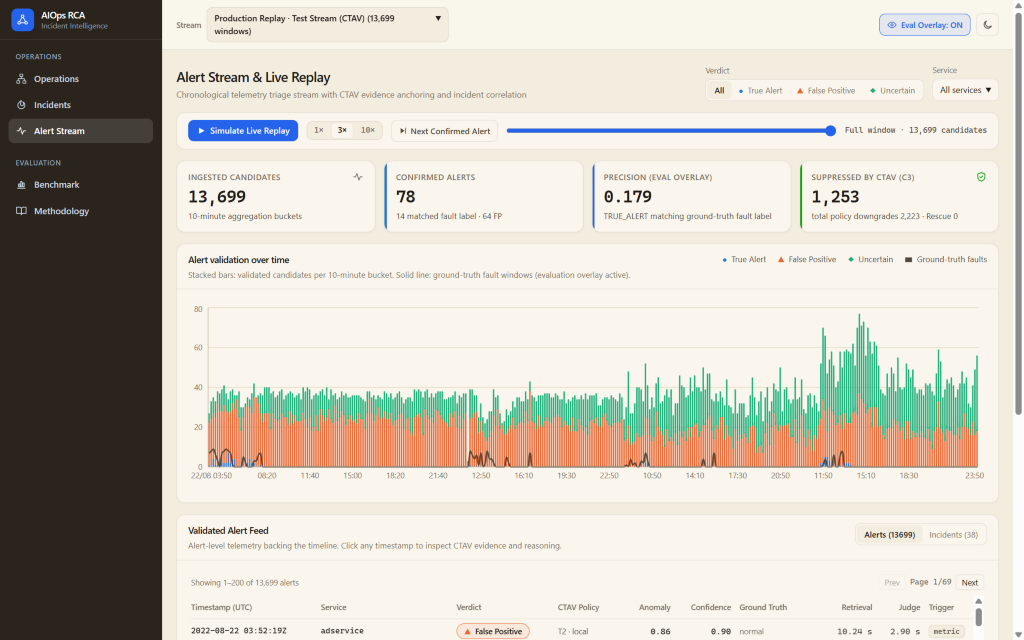
\includegraphics[width=\linewidth]{Images/C1/figures/m10-timeline.png}
  \par\vspace{0.4cm}
  \caption[Màn hình Alert Stream trên tập test]{Màn hình Alert Stream phát lại dòng phân loại $13.699$ cảnh báo đối chiếu nhãn chuẩn trên tập \splitname{test} (\code{pipeline\_test\_v2}).}
  \label{fig:ch6-timeline}
\end{figure}

Màn hình trả lời câu hỏi thứ hai của người vận hành: \emph{theo diễn tiến thời gian, lưu lượng cảnh báo ứng viên biến động ra sao và những cảnh báo xác nhận tập trung vào thời điểm nào?} Thanh điều khiển phát lại cho phép tua dòng cảnh báo từng bước ở tốc độ $1\times$, $3\times$, $10\times$ hoặc nhảy thẳng tới khung giờ có cảnh báo xác nhận kế tiếp (\emph{Next Confirmed Alert}), giúp tái hiện trực quan cách luồng cảnh báo đi qua bộ lọc \CTAV{} theo trật tự thời gian. Bên cạnh bảng cảnh báo phân trang 200 dòng, phân khu vận hành còn có màn hình hàng đợi sự cố chuyên biệt \emph{Incidents} (\code{/incidents}), nơi người trực ca lọc riêng các sự cố lan truyền đa service (\emph{Multi-service}) hoặc đơn service (\emph{Single-service}) và sắp xếp theo số lượng cảnh báo gom bên trong.

Nối với Chương~\ref{ch:de-xuat}, bốn thẻ chỉ số và biểu đồ cột phản ánh hiệu ứng kết hợp của ngưỡng \term{IF}{Isolation Forest}, bộ truy xuất \comp{C1} và cổng neo \comp{C3} (Mục~\ref{sec:ch4-policy}). Khi bật \emph{Eval Overlay}, màn hình cũng phơi bày trung thực giới hạn độ phủ mà Chương~\ref{ch:thuc-nghiem} đã chỉ ra: nhiều đỉnh của đường tiêm lỗi không có vạch xanh dương nào bên dưới. Đây chính là các đợt tiêm lỗi rơi vào nhóm $32/42$ service thiếu ngưỡng nền \splitname{dev}, nơi \comp{C3} hạ bậc toàn bộ cảnh báo do không có mốc tham chiếu cục bộ (Phát hiện 11, Mục~\ref{sec:ch5-finding11}).

\subsubsection{Alert Detail: vì sao giữ hay hạ một cảnh báo}
\label{sec:ch6-alert}

Hình~\ref{fig:ch6-alert} trình bày màn hình \emph{Alert Detail} của ứng viên \code{cand-ad327c0b162f6198} trên một cửa sổ bình thường của \code{productcatalogservice} (\code{pipeline\_test\_v2}). Người đọc nên đọc theo ba tầng từ trên xuống: hàng thẻ thông số và biểu đồ chuỗi điểm bất thường ở bên trái, lời giải thích của judge cùng bảng kiểm tra chính sách \CTAV{} ở cột phải, và thẻ giải thích ngữ cảnh \emph{How \comp{C1} built this context} trải rộng ở phần dưới.

\begin{figure}[htbp]
  \centering
  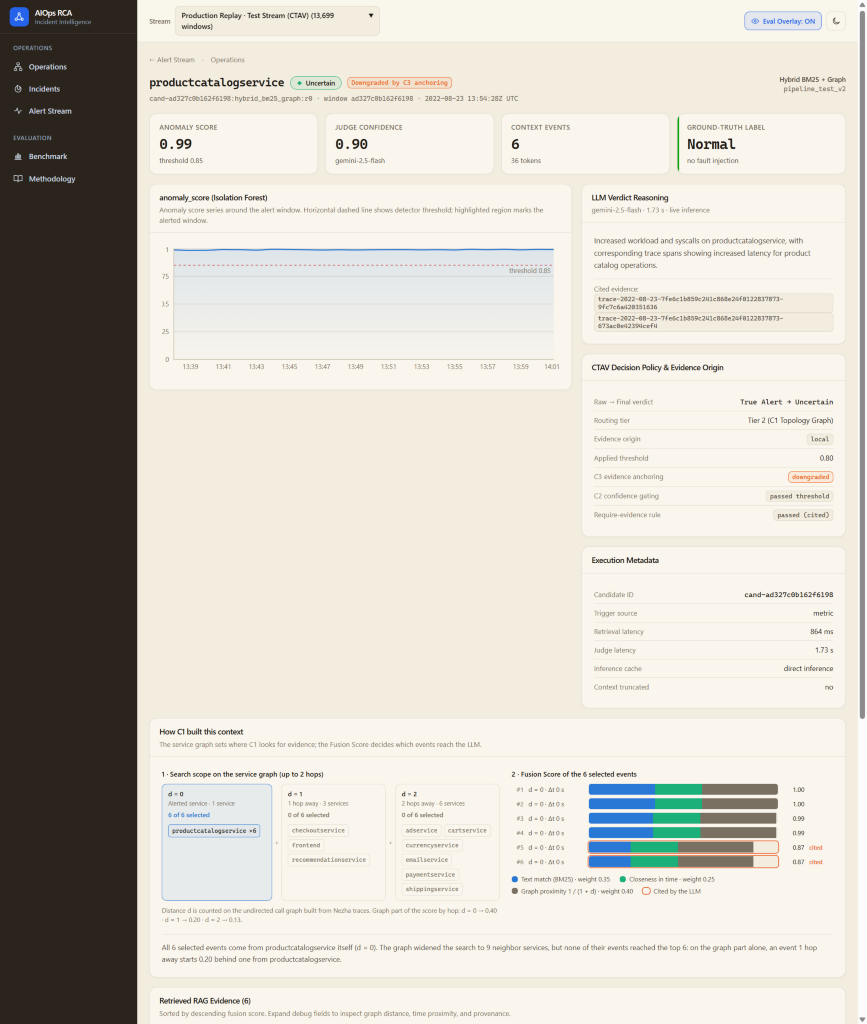
\includegraphics[width=\linewidth,height=0.72\textheight,keepaspectratio]{Images/C1/figures/m10-alert-c3-downgrade.png}
  \par\vspace{0.4cm}
  \caption[Màn hình Alert Detail giải thích ca bị C3 hạ bậc]{Màn hình Alert Detail giải thích ca báo động giả bị \comp{C3} hạ bậc và vùng ngữ cảnh \comp{C1} (\code{cand-ad327c0b162f6198}, \code{pipeline\_test\_v2}).}
  \label{fig:ch6-alert}
\end{figure}

Màn hình trả lời câu hỏi cốt lõi ở cấp độ từng cửa sổ: \emph{cùng mang điểm bất thường rất cao, vì sao hệ thống giữ lại cảnh báo này nhưng hạ bậc cảnh báo kia, và đồ thị phụ thuộc đã đóng góp gì vào bộ bằng chứng mà judge đọc?} Ở cột phải của Hình~\ref{fig:ch6-alert}, người vận hành thấy nguyên văn lập luận của \code{gemini-2.5-flash} viện dẫn hai span trace cục bộ để kết luận độ trễ tăng, tiếp theo là bảng thực thi tuần tự ba quy tắc chính sách: luật bắt buộc trích dẫn bằng chứng (\code{passed}), ngưỡng tin cậy $\theta = 0{,}80$ (\code{passed threshold}) và bước neo \comp{C3} (\code{downgraded}). Vì cả hai span được trích dẫn đều có thời gian thực thi nằm dưới phân vị $p_{90}$ của \splitname{dev}, \comp{C3} bác bỏ kết luận cảm tính của judge và hạ phán quyết xuống \code{Uncertain}. % src: m10_demo_cases_v1 step2

Đây là nơi cơ chế hiệu chỉnh của Mục~\ref{sec:ch4-policy} và \term{ConfirmationBias}{thiên lệch xác nhận} ở Phát hiện 7 (Bảng~\ref{tab:ch5-findings}) hiện ra trực tiếp trên dữ liệu thật. Thẻ \emph{How \comp{C1} built this context} ở nửa dưới Hình~\ref{fig:ch6-alert} giải thích minh bạch vai trò của đồ thị ở tầng truy xuất: nửa trái chia vùng tìm thành ba dải khoảng cách $d = 0, 1, 2$ trên đồ thị gọi vô hướng (tương ứng $1$, $3$ và $6$ service quanh \code{productcatalogservice}); nửa phải vẽ thanh thành phần \term{FusionScore}{Fusion Score} gồm $0{,}35 \times \mathrm{BM25}$, $0{,}25 \times$ độ gần thời gian và $0{,}40 \times 1/(1+d)$ đúng theo Công thức~\eqref{eq:ch4-fusion}, kèm viền cam quanh bằng chứng được judge trích dẫn. Cả sáu sự kiện lọt vào top-6 đều thuộc chính \code{productcatalogservice} ($d = 0$), vì một sự kiện cách 1 hop đã chịu mức phạt $0{,}20$ điểm ở thành phần đồ thị. Thẻ không tô vẽ kịch bản ``service lân cận cứu cảnh báo'', nhất quán với thực tế trên \code{pipeline\_test\_v2} chỉ có $75/19.794$ bằng chứng ($0{,}38\%$, thuộc $15/3.299$ cảnh báo có ngữ cảnh) đến từ service lân cận. % src: scripts/m11_graph_evidence_share.py --run-id pipeline_test_v2

\subsubsection{Incident Detail: định vị service gốc và đồ thị lân cận}
\label{sec:ch6-incident}

Hình~\ref{fig:ch6-incident} trình bày màn hình \emph{Incident Detail} của sự cố đa service \code{inc-46289ea526eaa3f3}, lấy từ luồng độ nhạy ngoài đăng ký \code{pipeline\_sens\_test\_v1} (biến thể \comp{C3} dùng ngưỡng nền trượt 60 phút) do lượt chạy đăng ký trên \splitname{test} không sinh ra cụm sự cố đa service nào. Người đọc nên chú ý hai dải băng vàng cảnh báo chế độ độ nhạy ở đầu trang, thẻ kể chuyện ba bước \emph{How the \term{RCA}{RCA} agent localized the root cause} ở giữa, cùng đồ thị lân cận ngang (\emph{Service Neighborhood Graph}) đặt cạnh báo cáo chẩn đoán JSON ở nửa dưới.

\begin{figure}[htbp]
  \centering
  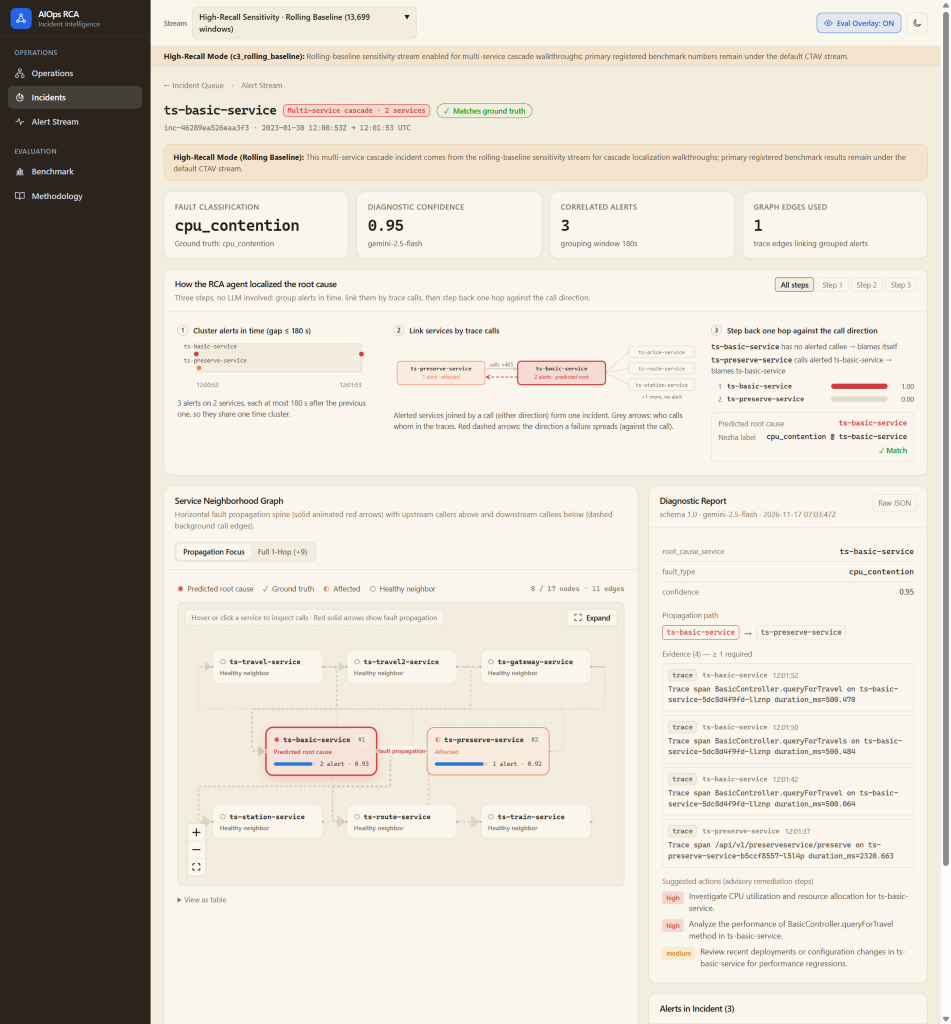
\includegraphics[width=\linewidth,height=0.72\textheight,keepaspectratio]{Images/C1/figures/m10-incident-cascade.png}
  \par\vspace{0.4cm}
  \caption[Màn hình Incident Detail định vị sự cố đa service]{Màn hình Incident Detail định vị service gốc ba bước và hiển thị đồ thị lan truyền của sự cố \code{inc-46289ea526eaa3f3} (\code{pipeline\_sens\_test\_v1}).}
  \label{fig:ch6-incident}
\end{figure}

Màn hình trả lời câu hỏi của khâu điều tra sự cố: \emph{khi nhiều cảnh báo nổ đồng thời trên các service liên kết nhau, lỗi phát sinh từ đâu, thuật toán suy diễn thứ hạng thế nào và gợi ý xử lý dựa trên bằng chứng nào?} Thẻ ba bước ở giữa tách bạch phần định vị hoàn toàn tất định (không dùng \term{LLM}{LLM}) thành ba khung có thể bấm chọn từng bước: (1)~trục thời gian gom ba cảnh báo trong khoảng cách $\le 180\,\text{s}$; (2)~sơ đồ các service có cảnh báo nối bởi mũi tên xám chỉ chiều gọi trong trace (\code{ts-preserve-service} gọi \code{ts-basic-service} $465$ lần) và mũi tên đỏ nét đứt chỉ chiều lỗi lan ngược, kèm các service hạ nguồn khỏe mạnh để thấy lý do dừng lan truyền; (3)~bảng chia phiếu bầu lùi một bước kết luận \code{ts-basic-service} đạt điểm tuyệt đối $1{,}00$, khớp nhãn gốc \code{cpu\_contention} của Nezha. % src: m10_demo_cases_v1 step4

Ở nửa dưới bên trái, đồ thị \emph{Service Neighborhood Graph} bố trí chuỗi lan truyền chính nằm ngang trên trục trung tâm (mũi tên đỏ liền nét từ \code{\#1 ts-basic-service} sang \code{\#2 ts-preserve-service}), tách các service gọi đến lên hàng trên và các service bị gọi xuống hàng dưới; chế độ mặc định \emph{Propagation Focus} giữ tối đa ba lân cận khỏe mạnh mỗi phía để sơ đồ thoáng rõ, có thể mở rộng toàn bộ qua nút \emph{Full 1-Hop (+9)} hoặc phóng toàn màn hình. Khung bên phải hiển thị báo cáo JSON đã vượt qua năm quy tắc kiểm duyệt ở Mục~\ref{sec:ch4-report}, gồm bốn trích đoạn trace kèm thời gian thực thi và ba khuyến nghị khắc phục phân mức ưu tiên. Như đã nhấn mạnh ở Mục~\ref{sec:ch5-rca-results}, ca này minh họa cơ chế gom và định vị của nhánh B vận hành đúng khi có đủ cảnh báo đầu vào, hoàn toàn không thay đổi kết luận \hyp{H5} không được chấp nhận trên luồng đăng ký chính thức ($38$ sự cố đơn service). % src: rca_final_test_v1

\subsubsection{Benchmark và Methodology: đối chiếu kiểm định và sổ tay phương pháp}
\label{sec:ch6-compare}

Hình~\ref{fig:ch6-compare} là màn hình \emph{Benchmark} (\code{/compare}), mặc định mở kết quả chính thức trên tập \splitname{test} và cho phép chuyển nhanh sang tập \splitname{val} để tham chiếu chéo. Dải cảnh báo vàng của luồng độ nhạy được tự động ẩn trên phân khu đánh giá để tránh gây nhầm lẫn với số liệu đăng ký. Người đọc nên nhìn bốn ô tóm tắt chỉ số đầu trang cùng cột trạng thái ba màu của bảng kiểm định \hyp{H0}--\hyp{H5}.

\begin{figure}[htbp]
  \centering
  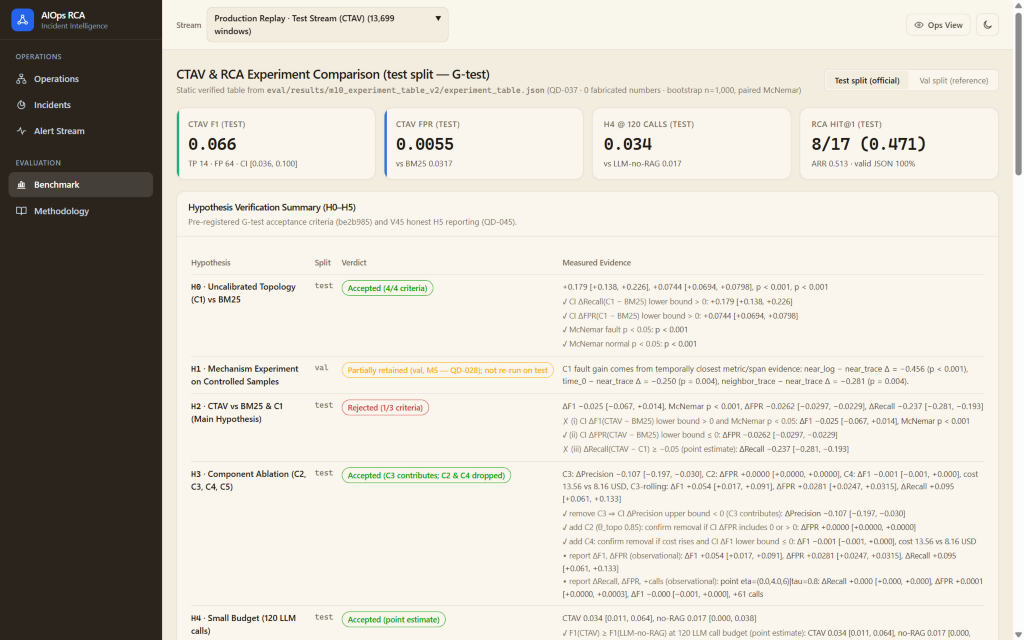
\includegraphics[width=\linewidth]{Images/C1/figures/m10-experiment-comparison.png}
  \par\vspace{0.4cm}
  \caption[Màn hình Benchmark tổng hợp kiểm định H0--H5]{Màn hình Benchmark (\code{/compare}) đối chiếu kết quả kiểm định \hyp{H0}--\hyp{H5} trên tập \splitname{test}.}
  \label{fig:ch6-compare}
\end{figure}

Màn hình trả lời câu hỏi của hội đồng thẩm định khoa học: \emph{khi đặt \CTAV{} cạnh các đường cơ sở theo đúng bản đăng ký giả thuyết trên \splitname{test}, giả thuyết nào được chấp nhận và giả thuyết nào bị bác bỏ?} Bên dưới bảng tổng hợp sáu giả thuyết là biểu đồ cột năm phương pháp kèm râu CI95 bootstrap, bảng hiệu ghép cặp kèm trị số $p$ của kiểm định McNemar, bảng ablation \hyp{H3} tích hợp điểm thử \comp{C5}, đường cong ngân sách \hyp{H4} và bảng kết quả \term{RCA}{RCA} của \hyp{H5} đặt cạnh dòng độ nhạy \code{C3-rolling}. Đi kèm màn hình này trong phân khu đánh giá là trang \emph{Methodology} (\code{/guide}), đóng vai trò sổ tay tra cứu tại chỗ trình bày trọn vẹn bốn công thức toán học của từng tầng xử lý, lý do loại bỏ các mô-đun âm (\comp{C2}, \comp{C4}, \comp{C5}) và bảng giải nghĩa thuật ngữ thống kê để phục vụ trực tiếp phiên hỏi đáp với hội đồng. Hai màn hình này nối thẳng với toàn bộ Chương~\ref{ch:thuc-nghiem} và là phiên bản tương tác của Bảng~\ref{tab:ch5-verdict-summary}.

% -----------------------------------------------------------------------------
\subsection{Kịch bản demo năm phút}
\label{sec:ch6-kich-ban}

Mục này chuẩn hóa kịch bản trình diễn năm bước trong thời lượng năm phút trước hội đồng. Toàn bộ mã ứng viên và mã sự cố trong kịch bản đều được rút tự động bằng quy tắc xác định (\code{seed = 42}) từ kho kết quả đã khóa của \splitname{test} và \splitname{val}, thay vì chọn thủ công; chẳng hạn ca ở bước 2 được lấy ngẫu nhiên có hạt giống từ tập $1.171$ cửa sổ bình thường trên \splitname{test} mà judge thô đánh nhãn \code{TRUE\_ALERT} nhưng bị \comp{C3} chặn lại. % src: m10_demo_cases_v1
Người trình bày có thể đi qua năm bước bằng cách bấm trực tiếp menu \emph{Guided Scenarios} ở chân thanh bên trái, giúp tự động đồng bộ đúng tham số \code{run\_id} và tự bật lớp phủ \emph{Eval Overlay} ở các bước đối chiếu nhãn.

Hai điểm điều chỉnh thực tế khi ánh xạ từ thiết kế sang dữ liệu thật được thuyết minh thẳng thắn ngay trong buổi demo. Thứ nhất, ở bước 3 về lỗi \code{network\_delay} mà \CTAV{} giữ được còn \term{BM25}{BM25} bỏ sót: trên \splitname{val}, \CTAV{} đánh rơi cả $10$ ca \code{network\_delay} của \comp{C1}, nhưng trên \splitname{test} có đúng $2$ ca thỏa mãn tiêu chí (\code{cartservice} và \code{ts-travel-service}). % src: ctav_final_val_v1, ctav_final_test_v1
Ở cả hai ca này, toàn bộ bằng chứng được chọn đều nằm ngay tại service phát cảnh báo ($d_G = 0$), nên thông điệp chính xác của bước 3 là \comp{C1} xếp hạng đúng span trễ cục bộ và \comp{C3} neo giữ thành công, chứ không phải ``nhờ log từ service lân cận''. Thứ hai, ở bước 4 về sự cố lan truyền nhiều service: luồng đăng ký \code{pipeline\_test\_v2} không có sự cố đa service nào, còn đợt tiêm lỗi \code{2023-01-30\#009} trên \code{pipeline\_val\_v2} lại bị tách thành hai sự cố đơn lẻ do service trung gian không phát cảnh báo để nối cạnh đồ thị. Kịch bản vì vậy chuyển sang luồng độ nhạy \code{pipeline\_sens\_test\_v1} (có dải băng vàng cảnh báo ngoài đăng ký) để trình diễn thuật toán định vị 3 bước, rồi đối chiếu ngay với ca bị tách đôi trên \splitname{val} để giải thích trực quan vì sao \hyp{H5} không đạt. Bảng~\ref{tab:ch6-kich-ban} tóm tắt năm bước thao tác.

\begin{table}[H]
  \centering
  \caption[Kịch bản demo năm phút trên giao diện điều hành]{Kịch bản demo năm phút trên bộ ca chọn tự động (\code{seed = 42}), chạy hoàn toàn ngoại tuyến với \code{DEMO\_OFFLINE=1}.}
  \label{tab:ch6-kich-ban}
  \tblfont
  \tblsetup
  \setlength{\tabcolsep}{3.5pt}
  \begin{tabularx}{\linewidth}{|>{\raggedright\arraybackslash}p{2.4cm}|>{\raggedright\arraybackslash}p{3.8cm}|Y|>{\raggedright\arraybackslash}p{3.3cm}|}
    \hline
    \rowcolor{gray!15}
    \textbf{Bước (thời lượng)} & \textbf{Thao tác} & \textbf{Người xem thấy} & \textbf{Thông điệp} \\
    \hline
    1. Toàn cảnh \& Dòng cảnh báo ($\approx 60$~s) & Mở \code{/overview} rồi sang \code{/timeline} của \code{pipeline\_test\_v2} (bật \emph{Eval Overlay}) & Bản đồ $56$ service ($5$ service có sự cố), chặn $96{,}6\%$ nhiễu thô ($2.223$ ca, riêng \comp{C3} hạ $1.253$ ca); còn $78$ \code{TRUE\_ALERT} $\to 38$ sự cố; tua nhanh thanh \emph{Live Replay} & Platform chạy khép kín ngoại tuyến ($4{,}24$~s từ cache); \CTAV{} nén mạnh báo động giả nhưng hụt đỉnh ở service thiếu ngưỡng \splitname{dev} \\
    \hline
    2. Chặn báo động giả nhờ \comp{C3} ($\approx 60$~s) & Chọn Kịch bản~2 (\code{cand-ad327c0b\allowbreak 162f6198}) mở Alert Detail & \code{productcatalogservice}, nhãn chuẩn \code{Normal}, điểm bất thường $0{,}99$; judge thô trả \code{True Alert} ($0{,}90$), thẻ chính sách ghi \comp{C3} hạ xuống \code{Uncertain}; thẻ \comp{C1} hiện đủ $6$ bằng chứng ở $d = 0$ & Neo định lượng $p_{90}$ chặn hiệu quả \term{ConfirmationBias}{thiên lệch xác nhận} trên trace cục bộ \\
    \hline
    3. Ca \code{network\_\allowbreak delay} \term{BM25}{BM25} bỏ sót ($\approx 60$~s) & Chọn Kịch bản~3 (\code{cand-fa85e82f\allowbreak 02f08574}) mở Alert Detail & \code{cartservice}: \term{BM25}{BM25} phán nhầm \code{False Positive} ($0{,}90$); \CTAV{} giữ \code{True Alert} nhờ span \code{CartService/GetCart} vượt ngưỡng \splitname{dev} (\code{anchored}); cả $6$ sự kiện ở $d = 0$ & \comp{C1} đưa đúng span trễ vào ngữ cảnh và \comp{C3} bảo toàn tín hiệu thật ($1$ trong $2$ ca trên \splitname{test}) \\
    \hline
    4. Sự cố cascade \& giới hạn \hyp{H5} ($\approx 75$~s) & Chọn Kịch bản~4 (\code{inc-46289ea5\allowbreak 26eaa3f3}, \code{pipeline\_sens\_\allowbreak test\_v1}); đối chiếu ca tách \code{2023-01-30\#009} trên \code{pipeline\_val\_v2} & Hai dải vàng ngoài đăng ký; thẻ 3 bước bỏ phiếu chấm \code{ts-basic-service} đạt $1{,}00$ khớp nhãn gốc; đồ thị trục ngang và JSON hợp lệ; trên \splitname{val} cùng đợt lỗi bị tách làm hai & Tác tử \term{RCA}{RCA} gom cụm và định vị đúng khi đủ cảnh báo; \hyp{H5} không đạt do độ phủ cảnh báo đầu vào thưa \\
    \hline
    5. Bảng kiểm định \& Sổ tay ($\approx 45$~s) & Mở \code{/compare} (chuyển thử \splitname{test}/\splitname{val}) và lướt \code{/guide} & Bảng \hyp{H0}--\hyp{H5} kèm CI95, đường cong ngân sách \hyp{H4}, bảng ablation \hyp{H3} + \comp{C5} và công thức bốn tầng ở \code{/guide} & \comp{C3} là đóng góp cốt lõi; \comp{C2}, \comp{C4} bị loại, \comp{C5} không mang lại lợi ích ròng; báo cáo trung thực cả \hyp{H2} và \hyp{H5} không đạt \\
    \hline
  \end{tabularx}
\end{table}

% -----------------------------------------------------------------------------
\subsection{Kiểm thử demo và dự phòng}
\label{sec:ch6-kiem-thu}

Mục này xác minh ba yêu cầu kỹ thuật của nền tảng trình diễn: vận hành hoàn toàn không cần Internet, bảo toàn tính nhất quán tuyệt đối với số liệu kiểm định, và có độ trễ khởi tạo đủ ngắn cho phiên bảo vệ. Bảng~\ref{tab:ch6-kiem-thu-dulieu} đối chiếu quy mô bản ghi, mức khớp kiểm chứng (\emph{parity}) và tỷ lệ trúng cache của ba lượt chạy được nạp vào cơ sở dữ liệu, còn Bảng~\ref{tab:ch6-kiem-thu-thoigian} phân rã thời gian thực thi đầu--cuối theo từng khâu. Cần lưu ý rằng thời gian trong Bảng~\ref{tab:ch6-kiem-thu-thoigian} là thời gian đọc lại từ cache trên đĩa và ghi vào hai kho lưu trữ, không phải độ trễ suy luận trực tuyến qua mạng; độ trễ gốc của từng lời gọi \term{LLM}{LLM} vẫn được bảo toàn nguyên vẹn trong ClickHouse để tra cứu ở màn hình Alert Detail.

\begin{table}[H]
  \centering
  \caption[Kiểm thử chạy ngoại tuyến: quy mô bản ghi, đối chiếu và cache]{Kiểm thử chạy ngoại tuyến của ba lượt chạy pipeline (phần 1): số bản ghi nạp, đối chiếu với kết quả kiểm định và tỷ lệ trúng cache.}
  \label{tab:ch6-kiem-thu-dulieu}
  \tblfont
  \tblsetup
  \setlength{\tabcolsep}{3.5pt}
  \begin{tabularx}{\linewidth}{|Y|>{\raggedright\arraybackslash}p{3.0cm}|>{\raggedright\arraybackslash}p{3.1cm}|>{\raggedright\arraybackslash}p{3.4cm}|}
    \hline
    \rowcolor{gray!15}
    \textbf{Chỉ số dữ liệu \& đối chiếu} & \textbf{\code{pipeline\_val\_v2} (\splitname{val})} & \textbf{\code{pipeline\_test\_v2} (\splitname{test})} & \textbf{\code{pipeline\_sens\_\allowbreak test\_v1} (\splitname{test}, độ nhạy ngoài ĐK)} \\
    \hline
    \code{candidate} nạp / \code{TRUE\_ALERT} & $5.677$ / $80$ & $13.699$ / $78$ & $13.699$ / $438$ \\
    \hline
    Dòng bằng chứng trong ClickHouse & $7.716$ & $19.794$ & $19.794$ \\
    \hline
    Sự cố / báo cáo hợp lệ (bị từ chối) & $26$ / $26$ ($0$) & $38$ / $38$ ($0$) & $114$ / $114$ ($0$) \\
    \hline
    Đối chiếu sự cố, thứ hạng, báo cáo với lượt kiểm định & $26/26$ & $38/38$ & $114/114$ \\
    \hline
    Lần gọi API mới / tỷ lệ trúng cache & $0$ / $100\%$ & $0$ / $100\%$ & $0$ / $100\%$ \\
    \hline
    Token judge trong cache (prompt / completion) & $5.173.670$ / $691.941$ & $12.736.820$ / $1.734.808$ & $12.736.820$ / $1.734.808$ \\
    \hline
  \end{tabularx}
\end{table}

\begin{table}[H]
  \centering
  \caption[Kiểm thử chạy ngoại tuyến: phân rã thời gian thực thi đầu--cuối]{Kiểm thử chạy ngoại tuyến của ba lượt chạy pipeline (phần 2): phân rã thời gian thực thi từng khâu khi nạp lại từ cache.}
  \label{tab:ch6-kiem-thu-thoigian}
  \tblfont
  \tblsetup
  \setlength{\tabcolsep}{3.5pt}
  \begin{tabularx}{\linewidth}{|Y|>{\raggedright\arraybackslash}p{3.0cm}|>{\raggedright\arraybackslash}p{3.1cm}|>{\raggedright\arraybackslash}p{3.4cm}|}
    \hline
    \rowcolor{gray!15}
    \textbf{Khâu thực thi} & \textbf{\code{pipeline\_val\_v2} (\splitname{val})} & \textbf{\code{pipeline\_test\_v2} (\splitname{test})} & \textbf{\code{pipeline\_sens\_\allowbreak test\_v1} (\splitname{test}, độ nhạy ngoài ĐK)} \\
    \hline
    Nạp cảnh báo và chính sách & $0{,}62$~s & $1{,}25$~s & $5{,}28$~s \\
    \hline
    Ghi ClickHouse & $2{,}90$~s & $1{,}27$~s & $2{,}79$~s \\
    \hline
    Gom sự cố và lan truyền & $4$~ms & $6$~ms & $19$~ms \\
    \hline
    Tóm tắt báo cáo (đọc cache) & $0{,}42$~s & $0{,}44$~s & $0{,}71$~s \\
    \hline
    Ghi PostgreSQL & $0{,}33$~s & $0{,}19$~s & $0{,}35$~s \\
    \hline
    \textbf{Tổng thời gian đầu--cuối} & $\mathbf{5{,}76}$~\textbf{s} & $\mathbf{4{,}24}$~\textbf{s} & $\mathbf{10{,}65}$~\textbf{s} \\
    \hline
  \end{tabularx}
\end{table}
% src: eval/results/{pipeline_val_v2,pipeline_test_v2,pipeline_sens_test_v1}/runtime.json
% Doi chieu: rca_final_val_v1, rca_final_test_v1, rca_sens_test_c3rolling_v1

Cả ba lượt chạy đều khớp $100\%$ với kết quả kiểm định gốc ở Chương~\ref{ch:thuc-nghiem} trên cả danh sách cảnh báo thành viên, thứ hạng service gốc lẫn mã băm nội dung báo cáo JSON, với $0$ lần gọi API mới. Luồng kiểm thử chính thức \code{pipeline\_test\_v2} hoàn tất nạp dữ liệu sau $4{,}24$~s, trong đó riêng thuật toán gom cụm và bỏ phiếu lan truyền của tác tử \term{RCA}{RCA} chỉ mất $6$~ms (và không quá $19$~ms ở luồng độ nhạy $438$ cảnh báo).

Kiểm thử vận hành thực tế được thực hiện ở hai lớp độc lập. Ở lớp kiểm thử tự động, bộ kiểm thử hợp đồng xác nhận toàn bộ tám endpoint (bao gồm \code{GET /topology}) trả đúng lược đồ dữ liệu trên cả ClickHouse lẫn PostgreSQL thật, kiểm chứng cơ chế xóa khóa API khi bật \code{DEMO\_OFFLINE=1}, đồng thời chạy bộ kiểm thử khói kết xuất phía máy chủ trên cả năm màn hình, các hàm suy diễn chính sách \comp{C3} và bộ xếp bố cục đồ thị. Ở lớp kiểm duyệt trình duyệt thật (tổng duyệt lần hai ngày 25/11/2026 sau khi nâng cấp giao diện điều hành), trình duyệt Chromium mở trực tiếp \code{http://localhost:5173} đi trọn năm màn hình của Bảng~\ref{tab:ch6-kich-ban}: toàn bộ trang tải hoàn tất với $0$ lỗi console, $0$ kết nối ra ngoài \code{localhost} và mọi truy vấn nội bộ đều trả mã HTTP 200. Các tồn đọng giao diện ghi nhận ở đợt tổng duyệt đầu tiên cũng đã được xử lý trọn vẹn: (i)~bộ hình Hình~\ref{fig:ch6-overview}--\ref{fig:ch6-compare} đã cập nhật đầy đủ thẻ giải thích \comp{C1}, thẻ ba bước \term{RCA}{RCA} và đồ thị phụ thuộc; (ii)~trục thời gian của Alert Stream tự động lặp lại tiền tố ngày \code{dd/MM} mỗi khi qua mốc nửa đêm; (iii)~dải băng vàng của luồng độ nhạy được cô lập khỏi phân khu đánh giá; và (iv)~mã nguồn giao diện được tách mảnh theo từng tuyến màn hình (\emph{code splitting}), giảm gói khởi tạo chính xuống còn khoảng $46$~kB ($\approx 16$~kB sau nén gzip) và triệt tiêu cảnh báo kích thước gói khi đóng gói. Trên thẻ phiếu bầu \term{RCA}{RCA}, $177/178$ sự cố của cả ba lượt chạy khớp trực tiếp điểm bầu từ cạnh gọi; duy nhất một sự cố hòa điểm $0{,}50$ được hệ thống phá hòa bằng điểm bất thường cực đại và gắn chú thích minh bạch ngay trên thẻ.

Phương án dự phòng cho buổi bảo vệ được thiết kế hai mức. Ở mức một, nếu một container gặp sự cố tức thời, lệnh \code{docker compose --profile dev up -d} khởi tạo lại dịch vụ mà không ảnh hưởng dữ liệu lưu bền vững trong volume. Ở mức hai, phòng trường hợp máy trình chiếu gặp trục trặc môi trường Docker, toàn bộ ba lượt chạy (\code{pipeline\_test\_v2}, \code{pipeline\_val\_v2}, \code{pipeline\_sens\_test\_v1}) đã được kết xuất sẵn sang ảnh chụp API tĩnh (\code{VITE\_DATA\_SOURCE=static}, đóng gói bảng \code{alerts} dạng cột nén giảm khoảng $65\%$ dung lượng cùng trọn bộ chi tiết sự cố, cảnh báo mẫu và đồ thị \code{topology}). Nhờ cơ chế này, toàn bộ năm màn hình của giao diện vẫn mở và tương tác trực tiếp được từ tệp tĩnh trên trình duyệt (hoặc bản triển khai tĩnh trên GitHub Pages) mà không cần Docker hay cơ sở dữ liệu chạy nền, bên cạnh bộ năm ảnh chụp độ phân giải 300~dpi lưu sẵn.

% -----------------------------------------------------------------------------
\subsection{Kết chương}
\label{sec:ch6-ket-chuong}

Chương này đã trình bày nền tảng trình diễn hiện thực hóa trọn vẹn chuỗi xử lý của đề tài, từ \code{candidate} của bộ phát hiện qua \CTAV{} và tác tử \term{RCA}{RCA} tới tám endpoint chỉ đọc và giao diện năm màn hình tách bạch giữa điều hành trực ca với đối chiếu kiểm định. Vì dùng chung đường ống thực thi với harness nghiên cứu, mọi con số và ca bệnh trên màn hình đều khớp $100\%$ với kết quả đã kiểm định ở Chương~\ref{ch:thuc-nghiem}, nạp lại hoàn toàn từ cache sau $4{,}24$--$10{,}65$~s mà không phát sinh bất kỳ lời gọi API hay kết nối mạng bên ngoài nào. Mỗi màn hình giải quyết một câu hỏi cụ thể và gắn trực tiếp với thiết kế ở Chương~\ref{ch:de-xuat}: Operations với bức tranh đồ thị phụ thuộc toàn hệ, Alert Stream với diễn tiến nén nhiễu theo thời gian, Alert Detail với cơ chế neo định lượng \comp{C3} và vùng tìm \comp{C1}, Incident Detail với ba bước định vị của tác tử \term{RCA}{RCA}, cùng Benchmark và Methodology với bảng kiểm định \hyp{H0}--\hyp{H5}. Kịch bản demo năm phút sử dụng bộ ca chọn tự động theo hạt giống cố định, đồng thời kết hợp chế độ snapshot tĩnh không phụ thuộc Docker để bảo đảm an toàn trình diễn ở mọi điều kiện phòng họp. Chương~\ref{ch:thao-luan} tiếp theo đi sâu phân tích cơ chế và phân loại toàn bộ các ca sai đứng sau những giới hạn đã quan sát trên nền tảng này.
